%!TEX program = pdflatex
%!BIB program = bibtex
\documentclass[12pt]{article}
\usepackage{geometry}
% \geometry{left=2.0cm,right=2.0cm,top=2.5cm,bottom=2.5cm}


\usepackage{times}
\usepackage{soul}
\usepackage{url}
\usepackage[hidelinks]{hyperref}
\usepackage[utf8]{inputenc}
\usepackage[small]{caption}
\usepackage{graphicx}
\usepackage{subfigure}
\usepackage{amsmath}
\usepackage{amsthm}
\usepackage{booktabs}
\usepackage{algorithm}
\usepackage{algorithmic}
\usepackage{lipsum}
\usepackage{multirow}  % for multirow command used in the table
\usepackage{setspace}
\usepackage{ulem}  % 用于添加下划线
\urlstyle{same}

\newtheorem{example}{Example}
\newtheorem{theorem}{Theorem}


\begin{document}
\setstretch{1.5}
\linespread{1}
\title{Response to Reviewers of TCSVT-07024-2021: A Simple and Strong Baseline for Universal Targeted Attacks on Siamese Visual Tracking}
\author{Zhenbang Li, Yaya Shi, Jin Gao, Shaoru Wang, \\Bing Li, Pengpeng Liang, Weiming Hu}
\date{}
\maketitle

\noindent Dear Editors:

We would like to express our heartfelt gratitude to you and the reviewers for the insightful and helpful comments. When we revised the paper, we carefully considered and followed all the comments and suggestions provided by you and the reviewers. To summarize, we have made the following revisions:

(1) We have added the advantages \& limitations of the proposed method after experimental analysis and the future work to the conclusion.

(2) We have carefully considered and followed all the comments and suggestions related to the clarity of the writing, and made the new material a thoroughly revised manuscript.

(3) We have added 3 papers published in the IEEE Transactions on Circuits and Systems for Video Technology, which are most closely related to our manuscript, and analysed what is distinctive / new about our current manuscript related to these previously published papers.

\uline{
Research topics related to adversarial attacks includes digital watermarking \cite{9343885}, 3D face presentation attacks \cite{9303455} and adversarial defense \cite{9169672}.
Xiong et. al. \cite{9343885} generate digital watermarking by slightly modifying the pixel values of videos frame to protect video content from unauthorized access. Compared with \cite{9343885}, our purpose of modifying pixel values of video frames is attacking the tracker, instead of detecting the illegal distribution of a digital movie.
Jia et. al. \cite{9294085} generate 3D face artifacts to fool the face recognition system. Compared with \cite{9294085}, our method directly modifies the input of the network instead of changing the input of cameras using 3D face artifacts.
Wang et. al. \cite{9169672} propose white-box attack/defense methods for image classifiers. Compared with \cite{9169672}, we focus on attacking the object tracking networks instead of the image classification networks.
}

% 4 高晋1 2021 是一个相关滤波算法
\uline{Liu et. al. \cite{9376997} propose a correlation filtering tracking algorithm based on the visual memory multi-template update strategy.}
% 5 高晋2 2021 是一个相关滤波算法
Liu et. al. \cite{9132673} construct a fuzzy aided detection module to boost the correlation filtering tracking system.

% 6 综述 2021
\uline{A comprehensive survey of the related trackers is beyond the scope of this paper, so we only briefly review two aspects that are most relevant to our work. Please refer to \cite{9339950} for A thorough survey on visual object tracking methods.}

(4) We have added a new experiment to attack in the YCbCr color space to reduce the perceptibility.

(5) We have added a new way to generate the fake trajectory.

We hope that our revised manuscript is now appropriate for publication in IEEE Transactions on Circuits and Systems for Video Technology. Specific responses to all the comments of each reviewer are included in the rest of this document and highlighted using bold font after the comments of each reviewer for the convenience of cross-reference. To make the changes easier to identify where necessary, we also have underlined most of the revised parts in the manuscript and provide an underlined version for the convenience of second review.\\[10pt]
\indent We are looking forward to your reply.\\[10pt]
\noindent Yours sincerely,\\
\noindent Zhenbang Li, Yaya Shi, Jin Gao, Shaoru Wang, Bing Li, Pengpeng Liang, Weiming Hu
\\
\\
\\
\noindent Dr. Jin Gao (Contact author)\\
\noindent National Laboratory of Pattern Recognition (NLPR)\\
\noindent Institute of Automation, Chinese Academy of Sciences (CASIA)\\
\noindent Address: No. 95, Zhongguancun East Road, Haidian District,\\
\noindent Beijing 100190, P. R. China\\
\noindent Email: jin.gao@nlpr.ia.ac.cn

%%%%%%%%%%%%%%%%% 审稿人 1 %%%%%%%%%%%%%%%%%
\newpage
{\centering\section*{Response Letter to Reviewer \#1}}
\noindent Dear Reviewer \#1:

Thank you very much for your thorough review. Your insightful comments are very helpful for us to improve the quality of the paper. According to your comments and suggestions, we have carefully and extensively revised the manuscript. The main revised parts are highlighted by underlines in the underlined version for your convenience. You will find that all your comments and suggestions are considered and followed. We hope that our revised manuscript is now appropriate for publication in IEEE Transactions on Circuits and Systems for Video Technology.
In addition, point-to-point responses to your comments are given below and highlighted using bold font in line with your comments in order to facilitate cross-referencing.\\[10pt]
\indent We are looking forward to your reply.\\[10pt]
\noindent Yours sincerely,\\
\noindent Zhenbang Li, Yaya Shi, Jin Gao, Shaoru Wang, Bing Li, Pengpeng Liang, Weiming Hu
\\
\\
\\
\noindent Dr. Jin Gao (Contact author)\\
\noindent National Laboratory of Pattern Recognition (NLPR)\\
\noindent Institute of Automation, Chinese Academy of Sciences (CASIA)\\
\noindent Address: No. 95, Zhongguancun East Road, Haidian District,\\
\noindent Beijing 100190, P. R. China\\
\noindent Email: jin.gao@nlpr.ia.ac.cn

\newpage
\textit{This paper addresses the task of attacking Siamese network-based trackers in a simple yet effective fashion. Unlike other methods that operate in the video-specific attacking regime (which resides on network inference for generating perturbations while tracking), this method is the first to perform universal targeted attacks for Siamese trackers utilizing both the translucent perturbation and the adversarial patch together. By adding the perturbation to the template and adding the patch to the search image while performing tracking, this work fools the Siamese trackers to the fake target region and thus makes them fail in tracking the real target object. Overall, this is an interesting paper, and it is well written and organized. As it is a resubmitted manuscript, I notice that the authors have made substantial changes to the previous manuscript, which are able to appropriately respond to the comments made by the previous reviewers. Although the template perturbation and adversarial patch are both easy to observe for human eyes as the previous reviewers have pointed out, and the SSIMs for them are also lower than the video-specific attacking method, e.g., FAN \cite{FAN}, this reviewer believes that this proposed new framework can be a new configuration of adversarial attack on visual tracking for its achieved balance between the attack efficiency and the perturbation perceptibility. This new configuration will attract increasing attention from the visual tracking attack community to study on more efficient attack methods.}

\textbf{Many thanks for your positive comments on the strength of our paper and thenovelty of the proposed attack method.}

%%%% 问题 1.1 %%%%
\textit{In addition, I suggest the authors add more experiments to demonstrate the practicability of the attack method when the ground truth box information is missing in the training data. The experimental results show that it is effective to use the predicted boxes instead of ground truth boxes for training perturbations.}

\textbf{This question needs to be discussed with Jin Gao.}

%%%% 问题 1.2 %%%%
\textit{A small question is that it will be better if the authors can provide some pseudo code for the untargeted attack and targeted attack processes in addition to the training process. This will facilitate the understanding of the attacking process while performing tracking.}

\begin{algorithm}[tb]
    \caption{Attack Process}
    \label{alg:algorithm_attack}
    \textbf{Input}: Imperceptible perturbation $\delta$, adversarial patch $p$, Siamese tracker $f$, video $V=\{I_i\}_1^T$, $b^{gt}_1$ is the position of the real target in the first frame. $B^{fake}=\{b^{fake}_i\}_1^{T}$ is the trajectory we hope the tracker to output.\\
    \textbf{Output}: $B^{pred}=\{b^{pred}_i\}_1^{T}$
    \begin{algorithmic}[1] %[1] enables line numbers
      \STATE Generate the clean template image $\textbf{z}_1$ according to $I_1$ and $b^{gt}_1$.
      \STATE Generate the perturbed template image $\tilde{\textbf z}_1=\textbf z_1+\delta$.
      \STATE Let $i = 2$.
    \WHILE{$i \le T$}
    \STATE Generate clean search image $\textbf{x}_i$ according to $I_i$ and $b^{pred}_{i-1}$.
    \STATE $b^{fake}_i=\{x_{0_i}, y_{0_i}, x_{1_i}, y_{1_i}\}$
    \STATE Generate the perturbed searach image $\tilde{\textbf x} = A_{\text{add}}(\textbf x, p_k, \{x_0, y_0, x_1, y_1\}).$
    \STATE $\textbf{C, R, Q} = f(\tilde {\textbf x}_i, \tilde{\textbf z}_1).$
    \STATE Generate the predicted bounding box $b^{pred}_t$ according to $\textbf{C, R, Q}$.
    \STATE $i = i + 1.$
    \ENDWHILE
    \STATE \textbf{return} $\delta_N, p_N.$
    \end{algorithmic}
  \end{algorithm}

\textbf{Both the targeted attack and untargeted attack process follow the same steps as shown in Alg. \ref{alg:algorithm_attack}. The difference between the target attack and the untargeted attack is the evaluation. For the targeted attack, we compare the AO between $B^{pred}=\{b^{pred}_i\}_1^{T}$ and $B^{fake}=\{b^{fake}_i\}_1^{T}$. For the untargeted attack, we compare the AO between $B^{pred}=\{b^{pred}_i\}_1^{T}$ and $B^{gt}=\{b^{gt}_i\}_1^{T}$.}

%%%% 问题 1.3 %%%%
\textit{In addition, the font size in Fig. 9 is too small to read on my computer, which needs to be improved.}

\newgeometry{left=1cm,right=1cm,top=1cm,bottom=1cm}

\begin{figure*}[t!]
  \renewcommand\thefigure{9}
  \begin{center}
    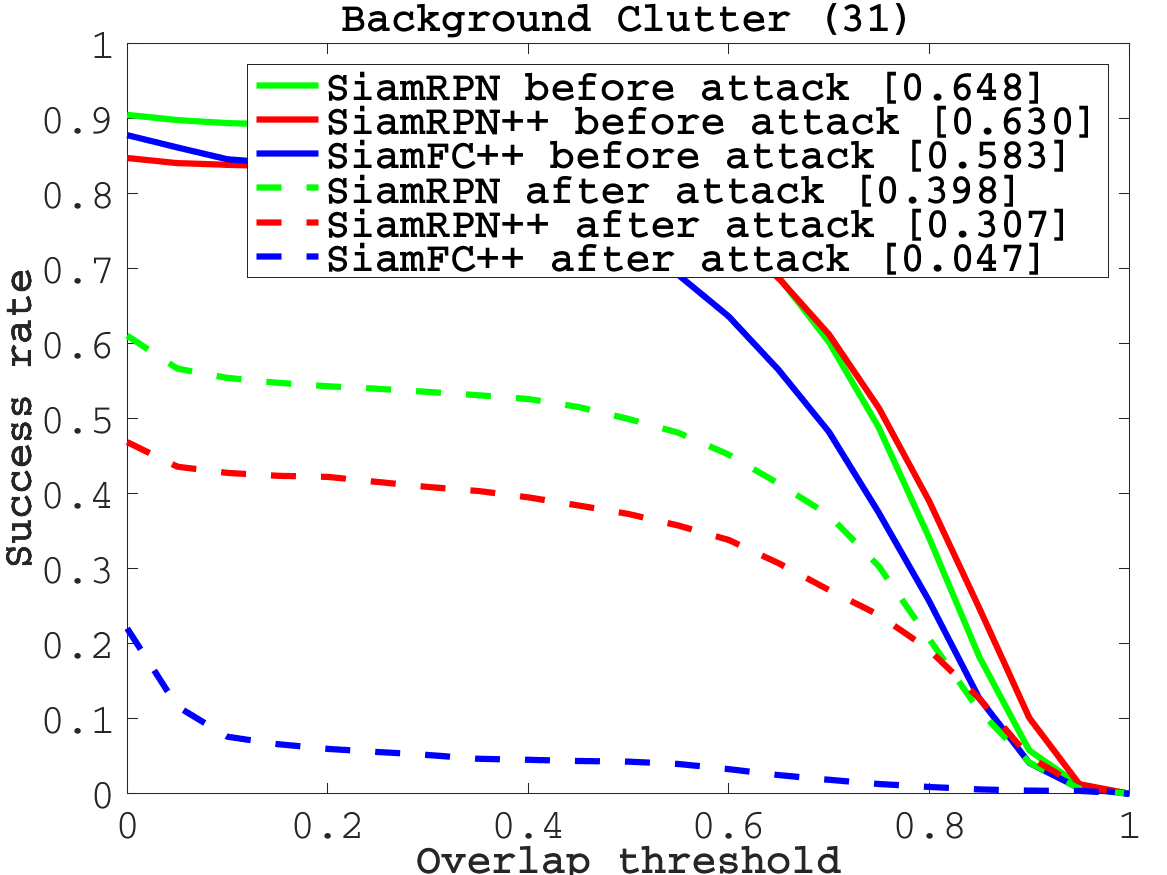
\includegraphics[width=0.32\textwidth]{images_imperceptible/OTB2015/success_plot_OPE_OTB100_BC.png}
    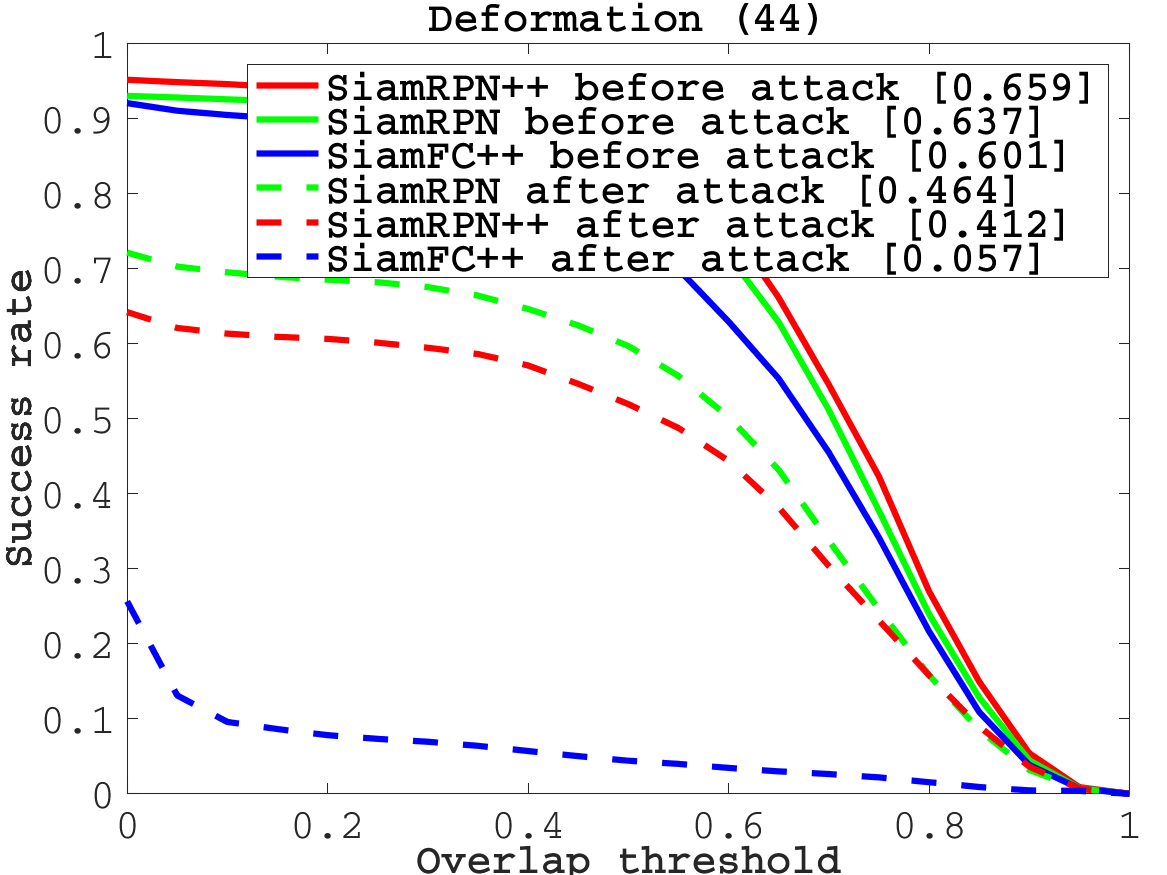
\includegraphics[width=0.32\textwidth]{images_imperceptible/OTB2015/success_plot_OPE_OTB100_DEF.png}
    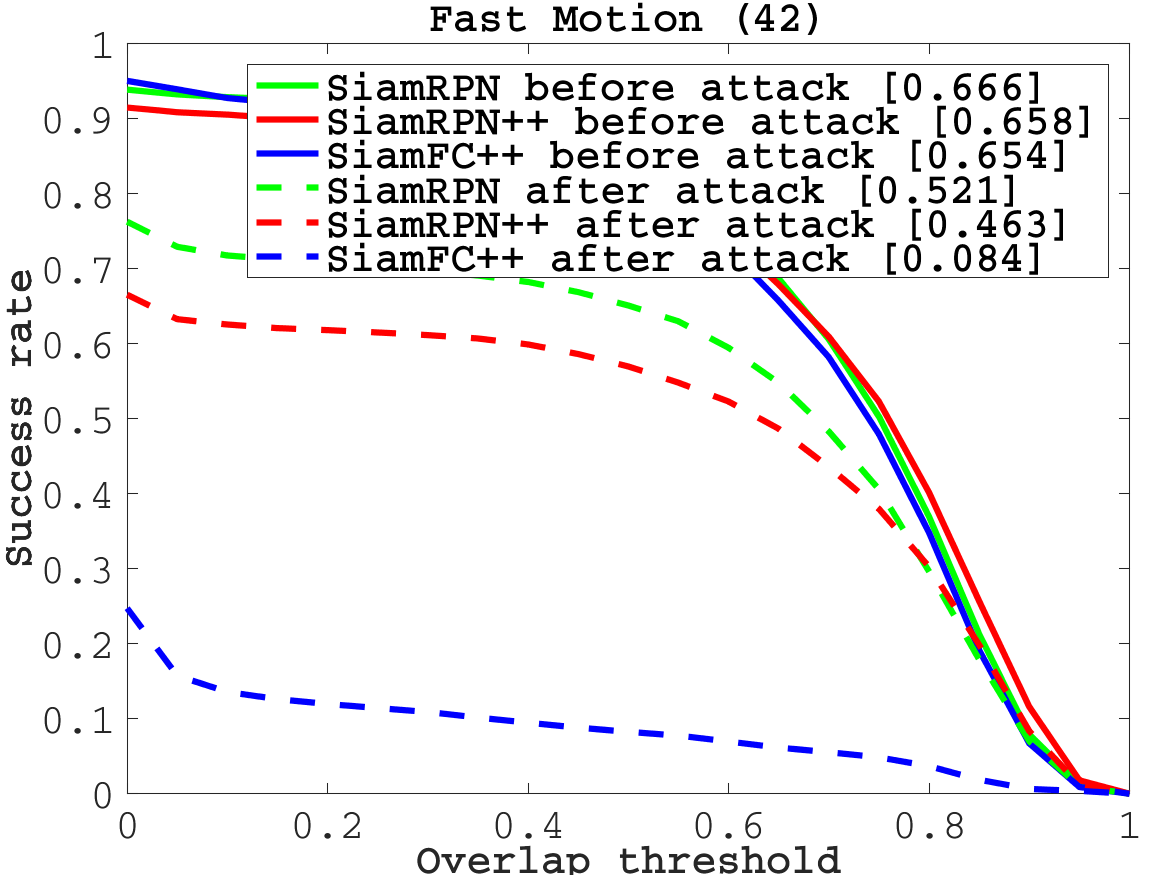
\includegraphics[width=0.32\textwidth]{images_imperceptible/OTB2015/success_plot_OPE_OTB100_FM.png}
    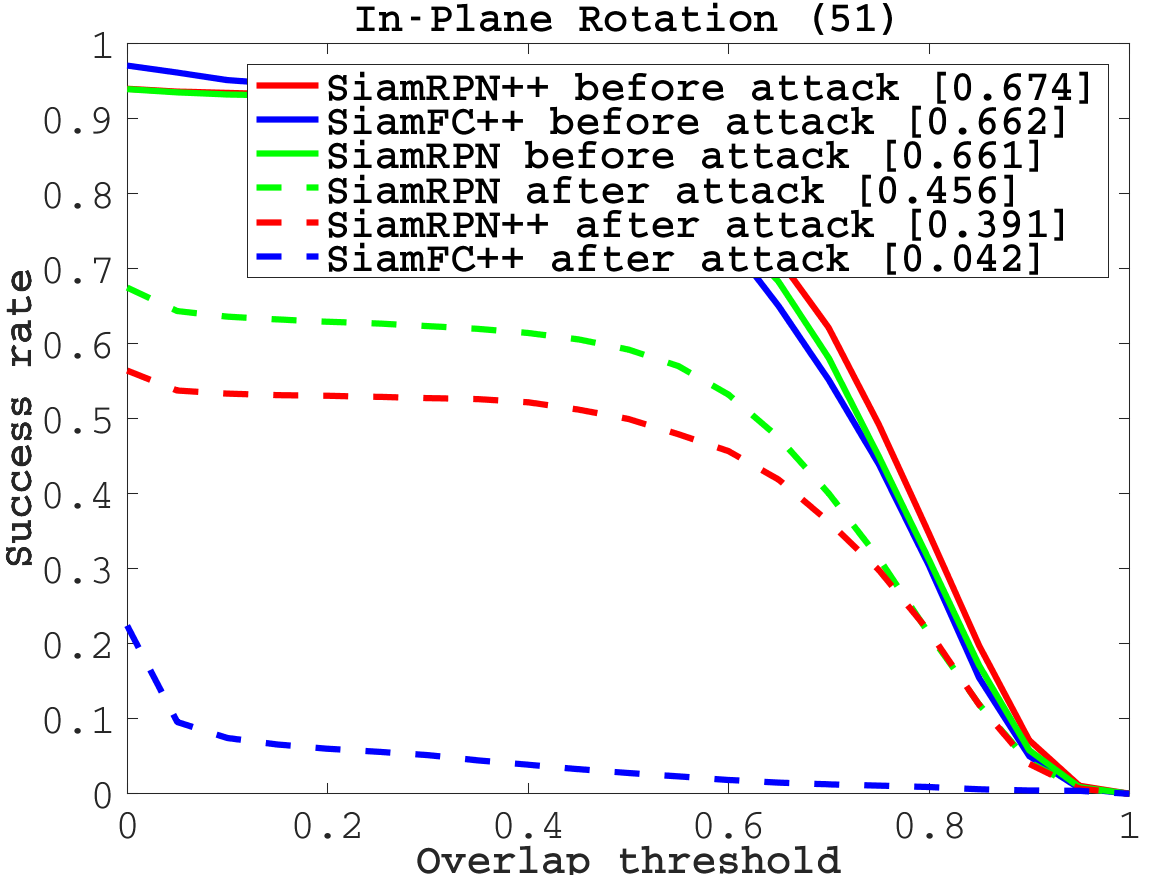
\includegraphics[width=0.32\textwidth]{images_imperceptible/OTB2015/success_plot_OPE_OTB100_IPR.png}
    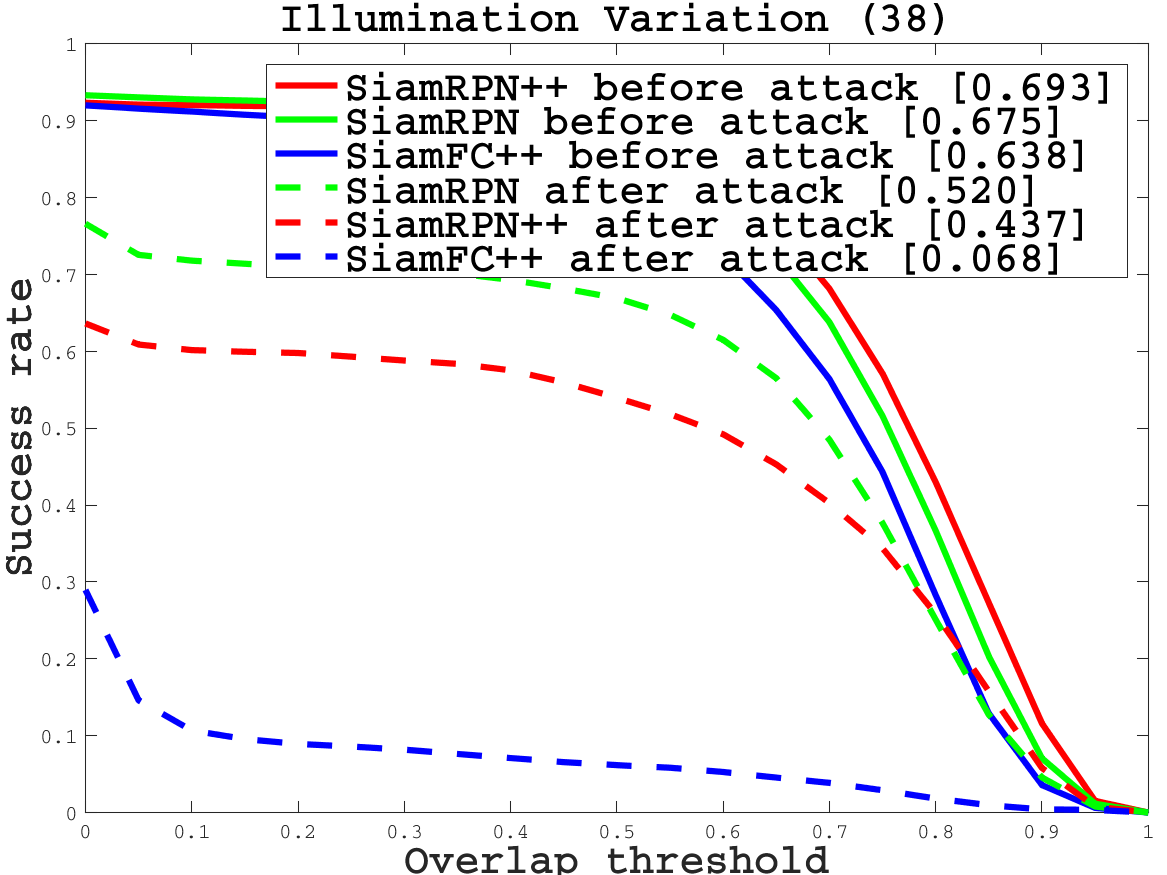
\includegraphics[width=0.32\textwidth]{images_imperceptible/OTB2015/success_plot_OPE_OTB100_IV.png}
    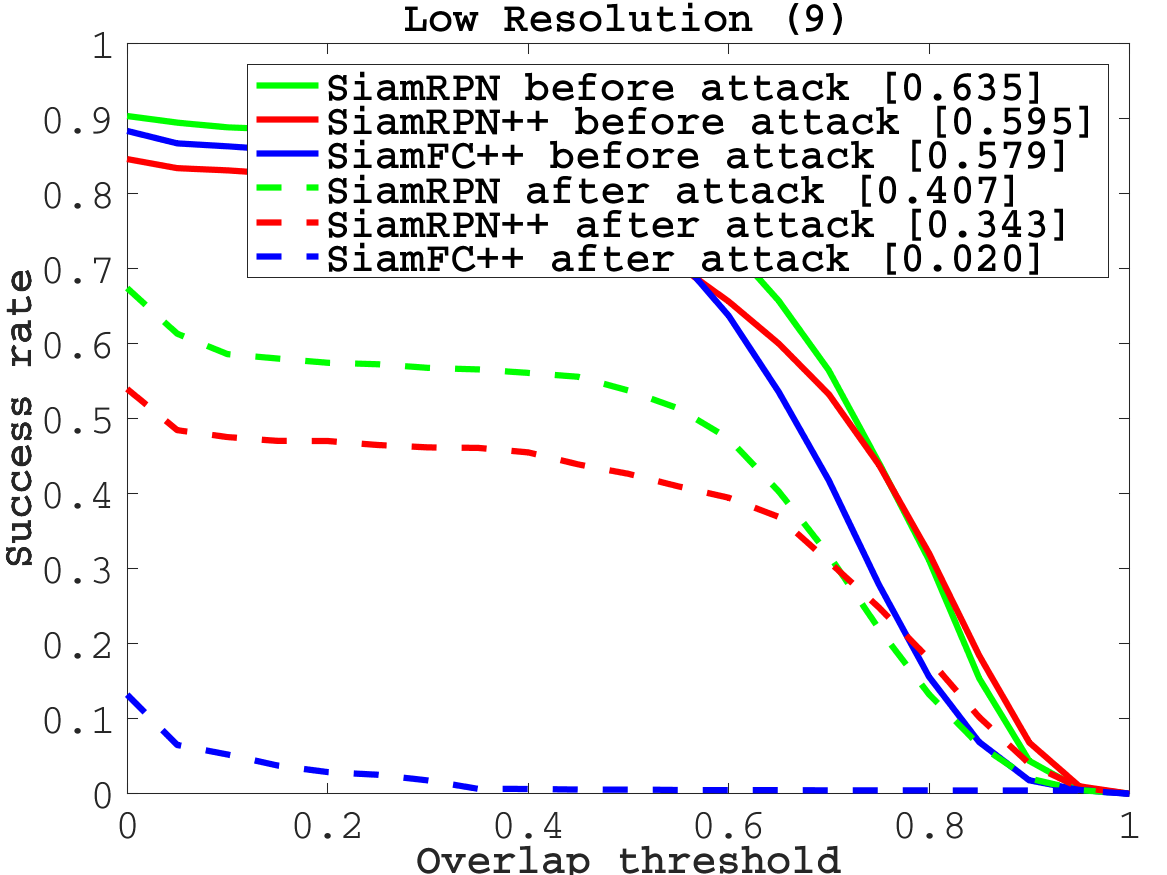
\includegraphics[width=0.32\textwidth]{images_imperceptible/OTB2015/success_plot_OPE_OTB100_LR.png}
    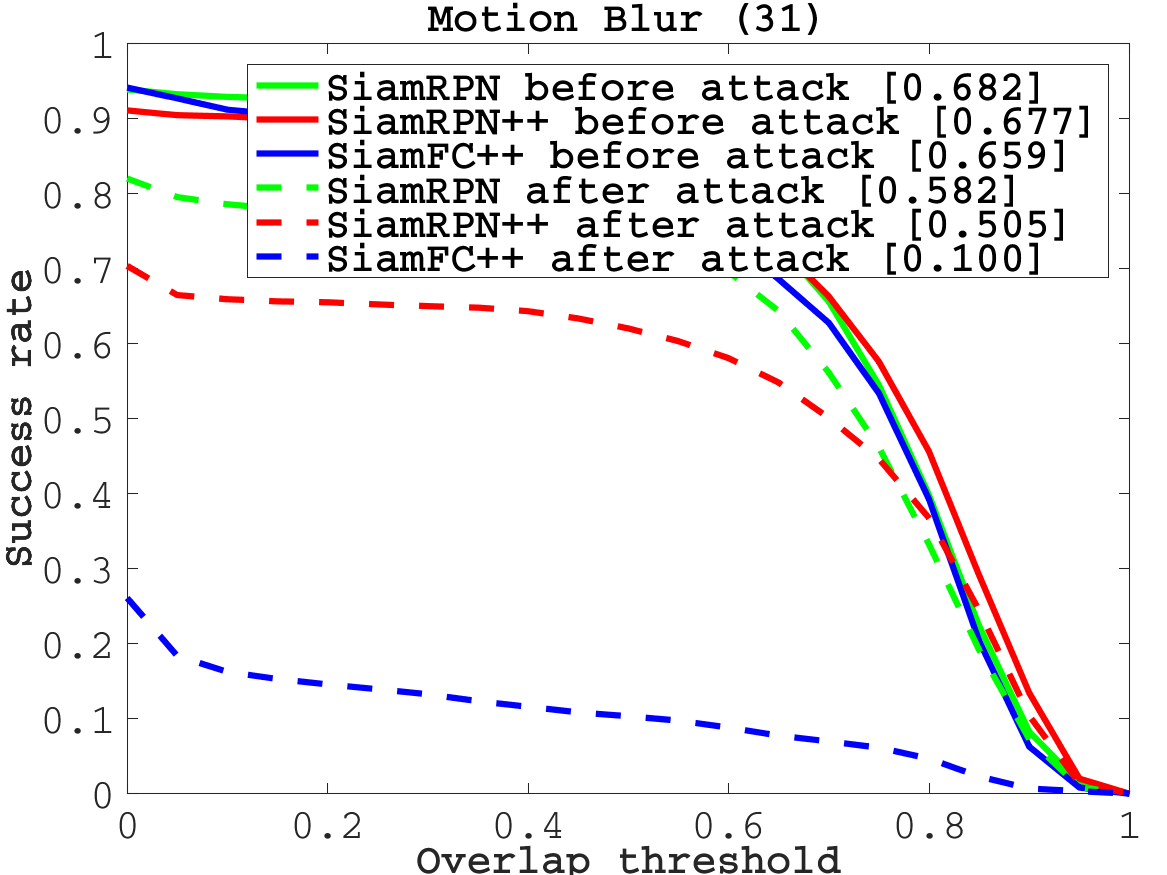
\includegraphics[width=0.32\textwidth]{images_imperceptible/OTB2015/success_plot_OPE_OTB100_MB.png}
    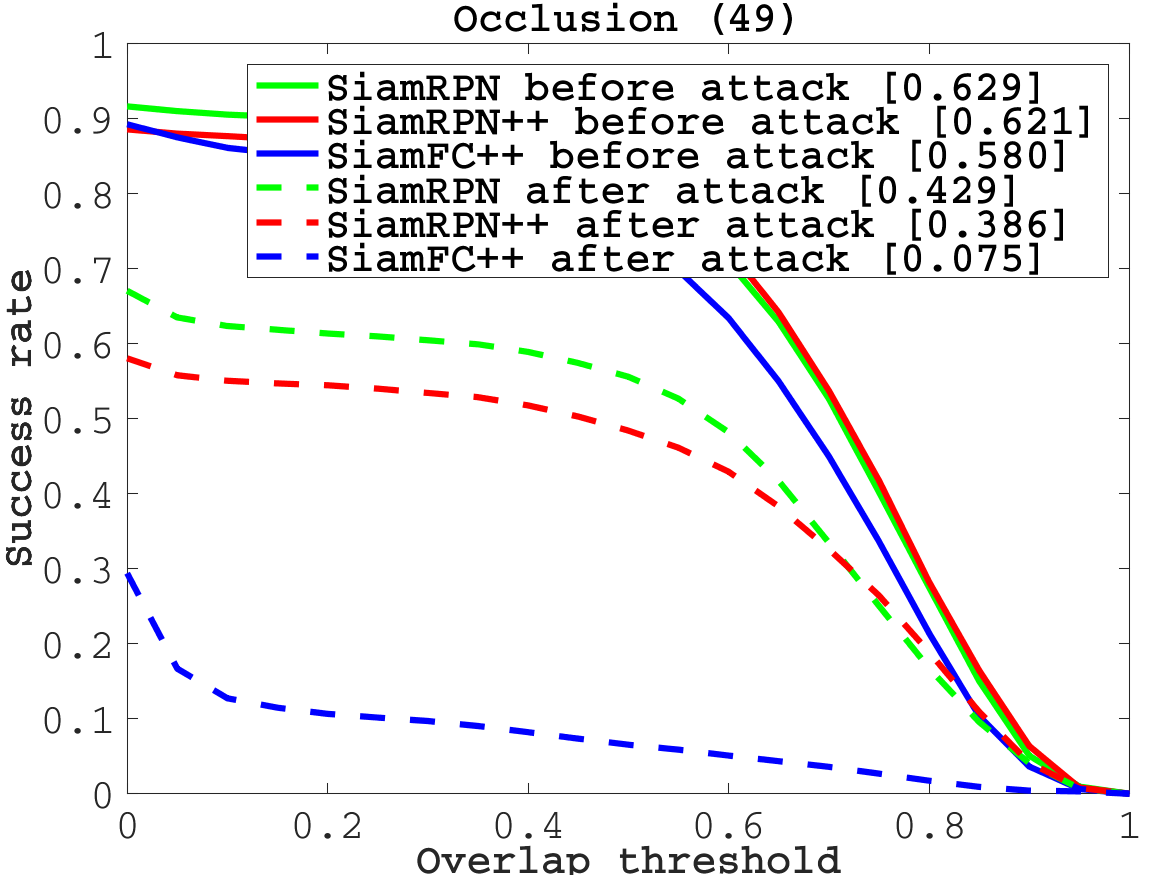
\includegraphics[width=0.32\textwidth]{images_imperceptible/OTB2015/success_plot_OPE_OTB100_OCC.png}
    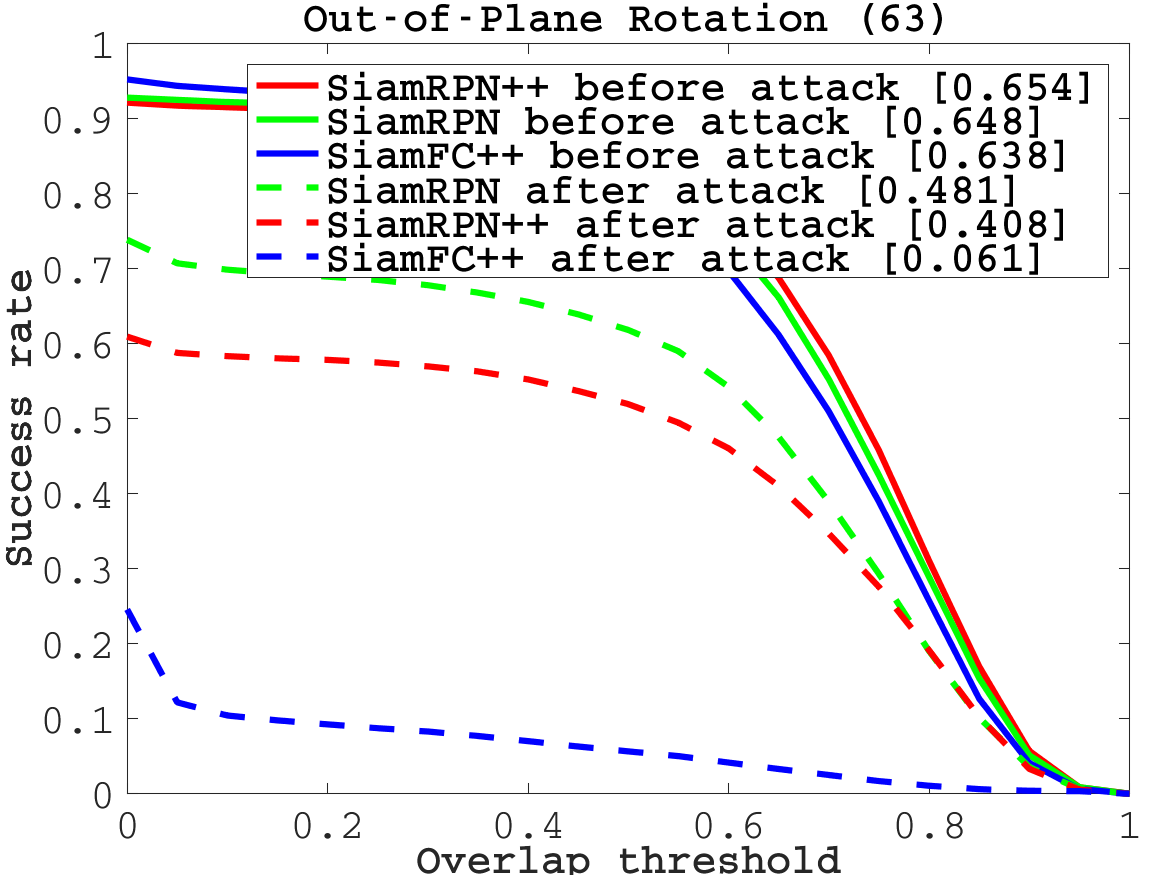
\includegraphics[width=0.32\textwidth]{images_imperceptible/OTB2015/success_plot_OPE_OTB100_OPR.png}
    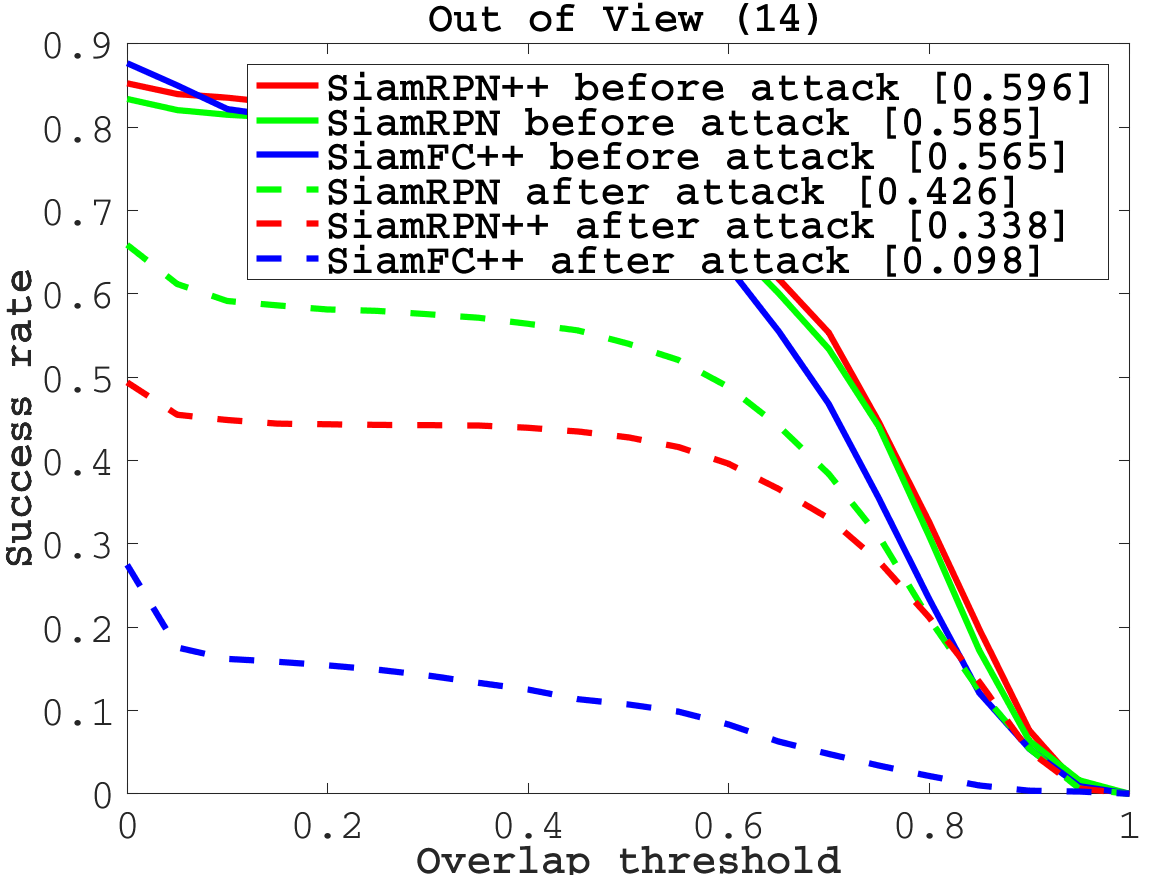
\includegraphics[width=0.32\textwidth]{images_imperceptible/OTB2015/success_plot_OPE_OTB100_OV.png}
    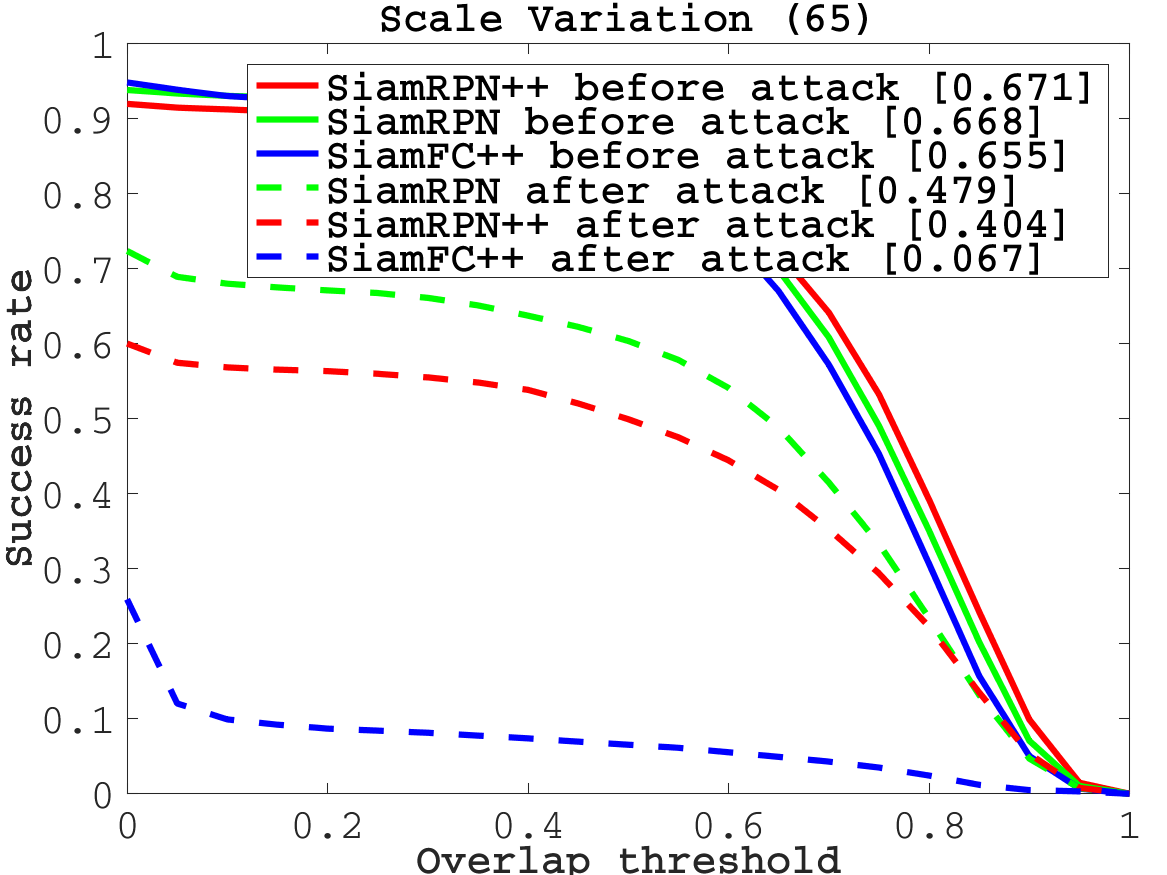
\includegraphics[width=0.32\textwidth]{images_imperceptible/OTB2015/success_plot_OPE_OTB100_SV.png}
  \end{center}
      \caption{Untargeted attack results of the different trackers under the 11 attributes: out-of-view (OV), occlusion (OCC), illumination variation (IV), out-of-plane rotation (OPR), scale variation (SV),deformation (DEF), low resolution (LR), fast motion (FM), background clutters (BC), motion blur (MB), and in-plane rotation (IPR). The results show good transferability of our attacks to different tracking architectures, even if the generated perturbations are applied to anchor-based trackers.}
  \label{fig:attr}
\end{figure*}

\restoregeometry

%%%% 问题 1.4 %%%%
\textit{Also, some recent papers are valued to be referred (2020-2021), to ehahnce the quality.}

\textbf{...}

\textit{Research topics related to adversarial attacks includes digital watermarking \cite{9343885}, 3D face presentation attacks \cite{9303455} and adversarial defense \cite{9169672}.
Xiong et. al. \cite{9343885} generate digital watermarking by slightly modifying the pixel values of videos frame to protect video content from unauthorized access. Compared with \cite{9343885}, our purpose of modifying pixel values of video frames is attacking the tracker, instead of detecting the illegal distribution of a digital movie.
Jia et. al. \cite{9294085} generate 3D face artifacts to fool the face recognition system. Compared with \cite{9294085}, our method directly modifies the input of the network instead of changing the input of cameras using 3D face artifacts.
Wang et. al. \cite{9169672} propose white-box attack/defense methods for image classifiers. Compared with \cite{9169672}, we focus on attacking the object tracking networks instead of the image classification networks.}

%%%%%%%%%%%%%%%%% 审稿人 2 %%%%%%%%%%%%%%%%%
\newpage
{\centering\section*{Response Letter to Reviewer \#2}}
\noindent Dear Reviewer \#2:

Thank you very much for your thorough review. Your insightful comments are very helpful for us to improve the quality of the paper. According to your comments and suggestions, we have carefully and extensively revised the manuscript. The main revised parts are highlighted by underlines in the underlined version for your convenience. You will find that all your comments and suggestions are considered and followed. We hope that our revised manuscript is now appropriate for publication in IEEE Transactions on Circuits and Systems for Video Technology.
In addition, point-to-point responses to your comments are given below and highlighted using bold font in line with your comments in order to facilitate cross-referencing.\\[10pt]
\indent We are looking forward to your reply.\\[10pt]
\noindent Yours sincerely,\\
\noindent Zhenbang Li, Yaya Shi, Jin Gao, Shaoru Wang, Bing Li, Pengpeng Liang, Weiming Hu
\\
\\
\\
\noindent Dr. Jin Gao (Contact author)\\
\noindent National Laboratory of Pattern Recognition (NLPR)\\
\noindent Institute of Automation, Chinese Academy of Sciences (CASIA)\\
\noindent Address: No. 95, Zhongguancun East Road, Haidian District,\\
\noindent Beijing 100190, P. R. China\\
\noindent Email: jin.gao@nlpr.ia.ac.cn

\newpage
\textit{In this paper, the authors train a universal adversarial patch to add on both template and search regions of a Siamese based tracker to deteriorate its original performance. The proposed perturbations are video-agnostic, leading to a low computational cost during attack. The experiment validations show that the proposed method achieves favorable attack results on OTB2015, GOT-10k, LaSOT, UAV123, VOT2016, VOT2018 and VOT2019. In addition, the generated perturbations transfer well on other Siamese trackers as well. The idea of this paper is interesting and the experiments are thorough.}

\textbf{Many thanks for your positive comments on the strength of our paper and the novelty of the proposed attack method.}

%%%% 问题 2.1 %%%%
\textit{However, there are some concerns over the implementation, performance and writing. 1. The authors state that training with Ep. 4 leads to an obvious patch on the images while using Eq.5 into the training process results in a less obvious patch. The reviewer considers that giving a constraint (e.g. $l_{\infty}$) on the $p_x$ in Eq.4 can make the perturbation imperceptible intuitively. Please give more analysis on this setting.
Besides, the reviewer hopes to know the reason why give an extra perturbation on the template region. The perturbations on template and search regions look similar, while the authors say that they are different. Please state the difference between the patch application operator on search examples and the operator on template examples.
In addition, the denotations of $A_{paste}$ in Eq.4 and $A_{add}$ in Eq.5 seem like the same one.
}

\textbf{
Thanks for the good comment.
Before analysis if giving constraint (e.g. $L_{\infty}$) on the $p_x$ in Eq.4 is really lead to imperceptible or not, let us first clarify the concept of the $A_{paste}$ and $A_{add}$, which is not tell good in the previous manuscript.}

\textbf{% 解释paste(说明不需要加 constraint)
$A_{paste}$ means that,
% we use the pixel value in in every place of the perturbation to replace the original image pixel value at the corresponding position.
% The final pixel value is changed from the original value to a new value.
in the region where the perturbation is pasted, the pixel values of the original image is replaced with the pixel values of the perturbation.
% 说明加了约束也没用。
% As a result, even though we add constraint to the perturbation and it is small, when we paste it to the image, it shows nearly black but not imperceptible.
Thus, even if we add constraints to the patch so that the perturbation values are small, when the patch is pasted to the image, it will look like an almost black region, which is obvious rather than imperceptible.
}

% 解释加法
\textbf{
The operator $A_{add}$ means to apply additive noise, where the injecting small perturbations into the image. Often need constraint. the injected noise are small and sometimes invisible. If we add a patch onto the image, the final pixel value is the original value plus a new value.}

\textbf{The operator $A_{\text{add}}(\textbf{x}, p_\textbf{x}, b^{fake}_{\textbf{x}})$ and $\textbf{z} + \delta_\textbf{z}$ is similar. The only difference is that, $A_{\text{add}}$ means add the perturbation to a specific region because the patch size is less than the image, while $+$ means add the perturbation to the full image because the size is the same.}

\textbf{For your convenience of cross checking, the new added text is shown as follows:}

\uline{
$A_{paste}$ means that, in the region where the perturbation is pasted, the pixel values of the original image is replaced with the pixel values of the perturbation.
% 解释加法
The operator $A_{add}$ means to apply additive noise, where the injecting small perturbations into the input samples. Often need constraint. the injected noise are small and sometimes invisible.  
}


%%%% 问题 2.2 %%%%
\textit{2. I agree with reviewer 3, the ground truth boxes are inaccessible to trackers during the inference. It seems that the authors use the ground truth boxes to generate the fake trajectory in lines 51-57 on page 7. Please clarify it.}

\textbf{We generate new trajectory without the test GT: we let the fake box run straight to border of the image, speed and derection is random.
For your convenience, the new text is added as following:}

\uline{
Let us now turn to targeted attacks. In this context, we consider two scenarios:
1. The attacker forces the tracker to follow a fixed direction. We illustrate this with 4 different directions, consisting of shifting the box by (3, 3) pixels in each consecutive frames, corresponding to the four directions 45, -45, 135, -135.
2. The attacker seeks for the tracker to follow a more complicated trajectory. ...
}

% \begin{table}[t]
%   \centering
%   \caption{rewrq}
%   \begin{tabular}{@{}rcccc@{}}
%   \toprule
%          & \multicolumn{2}{c}{Untargeted Attack} & \multicolumn{2}{c}{Targeted Attack} \\
%          & AO                & SR                & AO               & SR               \\ \midrule
%   track2 & 0.1747            & 0.1442            & 0.8448           & 0.8972           \\ \bottomrule        
%   \end{tabular}
% \end{table}

%%%% 问题 2.3 %%%%
\textit{3. For the experiments, the authors should conduct the ablation study on only adding perturbations on the template images or the search regions to show the impact of $p$ and $\delta$.}

\textbf{Thanks for your advice and we have conducted the ablation study on only adding perturbations on the template images or the search regions to show the impact of $p$ and $\delta$. As we can see, only use one of them is not useful, because they are trained together. For your convenience of cross review, the new text is given as follows.}

\uline{To see the impact of $p$ and $\delta$, we add the ablation study on only adding perturbations on the template images or the search regions. The result is shown in table \ref{table:one_branch}. Experiment results shows that only train in one branch is not useful. For the untargeted attack, the only template result is 0.50, the only search result is 0.71. While both attack is 0.**. For the targeted attack, the only template result is 0.16, the only search attack is 0.16, while both attack is 0.**.}

\begin{table}[]
  \centering
  \caption{Attack performance when only use the template/search perturbation.}
  \label{table:one_branch}
  \begin{tabular}{@{}rcccc@{}}
  \toprule
                & \multicolumn{2}{c}{Untargeted Attack} & \multicolumn{2}{c}{Targeted Attack} \\
                & AO                & SR                & AO               & SR               \\ \midrule
  Only Template & 0.5097            & 0.5669            & 0.1555           & 0.1064           \\
  Only Search   & 0.7137            & 0.8414            & 0.1599           & 0.1320           \\
  Both          &                   &                   &                  &                  \\
  \bottomrule
  \end{tabular}
\end{table}

%%%% 问题 2.4 %%%%
\textit{4. As reviewer 1 and reviewer 2 say, the perturbations added to template regions and research regions are not imperceptible, which may be helpful to misguide the tracker. The reviewer considers that adding a similar random pattern on the template and search regions to further illustrate the effectiveness of the proposed method.}

\textbf{To illustrate the effectiveness of the proposed method, we add a random pattern on the template and search regions: the mean value and standard deviation is the same as the template/search image.
For your convenience of cross checking, the new added text is show as follows:
%Specifically, the mean value of the template perturbation is ***, the standard deviation of the template image is ***. The mean value of the search patch is ***, the standard deviation of the search image is ***. We create the gaussian noise.
%'FGT-AO', 'FGT-SR-50', 'GT-AO', 'GT-SR-50'
%0.14250828600526147, 0.10118303356737521, 0.7604903420033434, 0.8957391555256324
%mean z=0.05680246651172638, std z=6.4726996421813965, mean x=-0.12454431504011154, std x=9.011011123657227
}

\begin{table}[t]
  \centering
  \caption{Attack performance using the gaussian random noise. The mean value is set to zero. The noise is added to both the template and the search image, position and size is the same of original setting. We not train.}
  \begin{tabular}{@{}rccccc@{}}
  \toprule
  \multirow{2}{*}[-2pt]{STD} & \multirow{2}{*}[-2pt]{SSIM}& \multicolumn{2}{c}{Untargeted Attack} & \multicolumn{2}{c}{Targeted Attack} \\ \cmidrule{3-6}
                             &                            & AO                & SR                & AO               & SR               \\ \midrule
  0.1 & 0.1747            & 0.1442            & 0.8448           & 0.8972           &       \\
  1.0 & 0.1747            & 0.1442            & 0.8448           & 0.8972           & \\
  10.0 & 0.1747            & 0.1442            & 0.8448           & 0.8972          & \\
  \bottomrule        
  \end{tabular}
  \label{table:noise}
\end{table}

\uline{\textit{Ablation Study: Attack performance of the random noise} To illustrate the effectiveness of the proposed method, we add a random pattern on the template and search regions: the mean value and standard deviation is the same as the template/search image. Attack performance using the gaussian random noise. The mean value is set to zero. The noise is added to both the template and the search image, position and size is the same of original setting. We not train.
% 实验结果的分析
As shown in Table \ref{table:noise}, if we add small or midiam noise, it will not the tracking performance. Only very large pattern will have affact, but the SSIM is evry small.
}

%%%% 问题 2.5 %%%%
\textit{
5. There are some minor problems, grammar errors and typos in this paper. The reviewer hopes the authors polish this paper again.}

\textit{- On page 2, ‘1016’ $\rightarrow$ ‘2016’ in line 56. There is a same one in line 47 on page 6.}

\textit{- The denotation of $B_x^{fake}$ in Eq.4 is not clear enough, even though it can be inferred by the later part.}

\textit{- On page 4, ‘imperceptible’ $\rightarrow$ ‘imperceptibly’ in line 57.}

\textit{- The reinitialization of VOT-toolkit should be mentioned in the part of ‘experimental setup’.}

\textit{- On page 7, ‘.(see Table I)’ is a typo.}

\textbf{Thanks for the good comment. We have carefully checked through the whole text and corrected the grammar mistakes and typos. Specifically,}
\textbf{We have replaced ``Experiment results on OTB2015 \cite{OTB}, GOT-10k \cite{GOT-10k}, LaSOT \cite{GOT-10k}, UAV123 \cite{UAV123}, VOT1016 \cite{VOT2016}, VOT2018 \cite{VOT2018} and VOT2019 \cite{VOT2019}. benchmarks demonstrate the effectiveness and efficiency of our approach.'' with}
``\uline{Experiment results on OTB2015 \cite{OTB}, GOT-10k \cite{GOT-10k}, LaSOT \cite{LaSOT}, UAV123 \cite{UAV123}, VOT2016 \cite{VOT2016}, VOT2018 \cite{VOT2018} and VOT2019 \cite{VOT2019}. benchmarks demonstrate the effectiveness and efficiency of our approach.}''
\textbf{in Section I of the revised manuscript.}

\textbf{We have replaced ``In SiamFC++, the tracker first transforms the paired reference frame $I_1$ and annotation $b_1^{gt}$ to get an template image $\textbf z_1$, and transforms the search frame $I_i$ to get the search image $\textbf x_i$ centered at the position estimated in the previous frame.'' with}
``\uline{In SiamFC++, the tracker first transforms the paired reference frame $I_1$ and annotation $b_1^{gt}$ to get a template image $\textbf z_1$, and transforms the search frame $I_i$ to get the search image $\textbf x_i$ centered at the position estimated in the previous frame.}''
\textbf{in Section III.A of the revised manuscript.}

\textbf{We have replaced ``However, CNN attacks are usually expected imperceptible but the above method has to paste an obviously noticeable fake target patch to tracking frames, which raises the risk of being suspected.'' with}
``\uline{However, CNN attacks are usually expected imperceptibly but the above method has to paste an obviously noticeable fake target patch to tracking frames, which raises the risk of being suspected.}''
\textbf{in Section III.A of the revised manuscript.}

\textbf{We have  replaced ``$A_add$ adds the patch into the search image $\textbf x$ at location $(\frac{x_0+x_1}{2},\frac{y_0+y_1}{2})$.'' with}
``\uline{$A_{add}$ adds the patch into the search image $\textbf x$ at location $(\frac{x_0+x_1}{2},\frac{y_0+y_1}{2})$.}''
\textbf{in Section III.B of the revised manuscript.}

\textbf{We have replaced ``We evaluate our video-agnostic perturbations for targeted attacks on several tracking benchmarks, i.e., OTB2015 \cite{OTB}, GOT-10k \cite{GOT-10k}, LaSOT \cite{LaSOT}, UAV123 \cite{UAV123}, VOT1016 \cite{VOT2016}, VOT2018 \cite{VOT2018} and VOT2019 \cite{VOT2019}.'' with}
``\uline{We evaluate our video-agnostic perturbations for targeted attacks on several tracking benchmarks, i.e., OTB2015 \cite{OTB}, GOT-10k \cite{GOT-10k}, LaSOT \cite{LaSOT}, UAV123 \cite{UAV123}, VOT2016 \cite{VOT2016}, VOT2018 \cite{VOT2018} and VOT2019 \cite{VOT2019}.}''
\textbf{in Section IV.A of the revised manuscript.}

\textbf{We have replaced ``We adopt COCO \cite{COCO}, ILSVRC-VID \cite{VID} and the training splits of GOT-10k \cite{GOT-10k} and LaSOT \cite{LaSOT} as our training set. (see Table \ref{tab:dataset})'' with}
``\uline{We adopt COCO \cite{COCO}, ILSVRC-VID \cite{VID} and the training splits of GOT-10k \cite{GOT-10k} and LaSOT \cite{LaSOT} as our training set.}''
\textbf{in Section IV.B of the revised manuscript.}

%%%%%%%%%%%%%%%%% 审稿人 3 %%%%%%%%%%%%%%%%%
\clearpage
\newpage
{\centering\section*{Response Letter to Reviewer \#3}}
\noindent Dear Reviewer \#3:

Thank you very much for your thorough review. Your insightful comments are very helpful for us to improve the quality of the paper. According to your comments and suggestions, we have carefully and extensively revised the manuscript. The main revised parts are highlighted by underlines in the underlined version for your convenience. You will find that all your comments and suggestions are considered and followed. We hope that our revised manuscript is now appropriate for publication in IEEE Transactions on Circuits and Systems for Video Technology.
In addition, point-to-point responses to your comments are given below and highlighted using bold font in line with your comments in order to facilitate cross-referencing.\\[10pt]
\indent We are looking forward to your reply.\\[10pt]
\noindent Yours sincerely,\\
\noindent Zhenbang Li, Yaya Shi, Jin Gao, Shaoru Wang, Bing Li, Pengpeng Liang, Weiming Hu
\\
\\
\\
\noindent Dr. Jin Gao (Contact author)\\
\noindent National Laboratory of Pattern Recognition (NLPR)\\
\noindent Institute of Automation, Chinese Academy of Sciences (CASIA)\\
\noindent Address: No. 95, Zhongguancun East Road, Haidian District,\\
\noindent Beijing 100190, P. R. China\\
\noindent Email: jin.gao@nlpr.ia.ac.cn

\newpage

%%%% 问题 3.1 %%%%
\textit{This paper employs the universal perturbation attacks on Siamese visual trackers. There are still the following concerns about the proposed method. 1. As stated in the paper, the proposed method ``does not require gradient optimization or network inference". However, this is a double-edged sword since it resulted in suspicious attacks. Prior works commonly train a network to prevent not only suspicious attacks but also modifying every pixel. I think it's a major problem with this work. I suggest considering a proper strategy to remove/reduce it.}

\textbf{
Thanks for your advice.
% 承认已有问题:相比于现有的目标跟踪攻击算法,我们方法的不足之处是扰动值较为显眼。
The shortcoming of our method is the more conspicuous perturbation values compared to existing target tracking attack algorithms.
% 解释我们的扰动显眼的原因:其他方法在整个搜索图像添加扰动,而我们必须要在64*64这个很小的区域内添加扰动,这增加了学习的难度,使得扰动值大。
Other methods add perturbations over the entire search image, whereas we have to add perturbations over a very small region of 64*64, which increases the learning difficulty and makes the perturbation values large.
% 解释我们不用全图攻击的原因:我们仅在小区域内而不是在整个搜索图像上添加扰动,因为必须指定轨迹在哪。
% 解决方案:为了既享受全图扰动带来的低感知性,以及局部扰动用于指定目标位置,我们考虑在不同的图像通道执行不同的扰动:首先将图像转为YCbCr通道,在Y通道做全图攻击,在CbCr通道做局部攻击。or: 为了在有目标攻击的同时降低可感知性,...
To reduce perceptibility while having a targeted attack, we consider a new way to perturb the search image: first we convert the search image into YCbCr color space, then add pereturbations over the entire search image in the Y channel, and add perturbations over a very small region of 64*64 in the CbCr channel.
% 介绍什么是 YCbCr
Different from RGB color space, YCbCr color space encodes a color image similar to human eyes’ retina, which separates the RGB components into a luminance component (Y) and two chrominance components (Cb as blue projection and Cr as red projection).
% 解释为什么用YCbCr而不是RGB。选择 YCbCr 而不是 RGB 的原因是更加独立。
We choose YCbCr color space since its color channels are less correlated and quite independent than RGB.
% 解释为什么在CbCr上做局部攻击在Y上做全图攻击,而不是其他方式:有研究证明Y通道可感知性更强而CbCr弱一些。因为我们希望补丁区域扰动值更小,所以我们在CbCr做局部攻击。
While considering the color sensitivity of HVS, the CbCr channels are least sensitive that the Y channel. This means that the patch added in the CbCr channels has better performance of transparency.
% 实验细节:迭代了多少次?损失函数各项的权重是什么?模板图像怎么操作。
% 实验结果。
The experimental result is shown in Table. As we can see, ...
For your convenience of cross checking, the new next is added as following.
}

\begin{figure}[t]
  \centering
  \subfigure[SSIM=0.85]{\label{fig:a}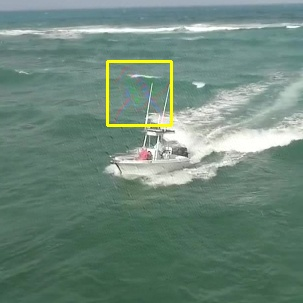
\includegraphics[width=0.15\textwidth]{images_imperceptible/2_adv_search_img_fgt.jpg}}
  \subfigure[SSIM=0.56]{\label{fig:a1}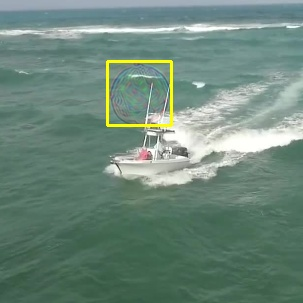
\includegraphics[width=0.15\textwidth]{images_imperceptible/64.jpg}}
  \subfigure[SSIM=0.79]{\label{fig:b}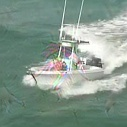
\includegraphics[width=0.15\textwidth]{images_imperceptible/16384_adv_template_img.jpg}}
  \subfigure[SSIM=0.79]{\label{fig:b}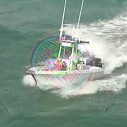
\includegraphics[width=0.15\textwidth]{images_imperceptible/template.jpg}}
  \caption{YCbCr Attack.}
  \label{fig:patch_size_vis}
\end{figure}

\uline{
% 承认已有问题:相比于现有的目标跟踪攻击算法,我们方法的不足之处是扰动值较为显眼。
The shortcoming of our method is the more conspicuous perturbation values compared to existing target tracking attack algorithms.
% 解释我们的扰动显眼的原因:其他方法在整个搜索图像添加扰动,而我们必须要在64*64这个很小的区域内添加扰动,这增加了学习的难度,使得扰动值大。
Other methods add perturbations over the entire search image, whereas we have to add perturbations over a very small region of 64*64, which increases the learning difficulty and makes the perturbation values large.
% 解释我们不用全图攻击的原因:我们仅在小区域内而不是在整个搜索图像上添加扰动,因为必须指定轨迹在哪。
% 解决方案:为了既享受全图扰动带来的低感知性,以及局部扰动用于指定目标位置,我们考虑在不同的图像通道执行不同的扰动:首先将图像转为YCbCr通道,在Y通道做全图攻击,在CbCr通道做局部攻击。or: 为了在有目标攻击的同时降低可感知性,...
To reduce perceptibility while having a targeted attack, we consider a new way to perturb the search image: first we convert the search image into YCbCr color space, then add pereturbations over the entire search image in the Y channel, and add perturbations over a very small region of 64*64 in the CbCr channel.
% 介绍什么是 YCbCr
Different from RGB color space, YCbCr color space encodes a color image similar to human eyes’ retina, which separates the RGB components into a luminance component (Y) and two chrominance components (Cb as blue projection and Cr as red projection).
% 解释为什么用YCbCr而不是RGB。选择 YCbCr 而不是 RGB 的原因是更加独立。
We choose YCbCr color space since its color channels are less correlated and quite independent than RGB.
% 解释为什么在CbCr上做局部攻击在Y上做全图攻击,而不是其他方式:有研究证明Y通道可感知性更强而CbCr弱一些。因为我们希望补丁区域扰动值更小,所以我们在CbCr做局部攻击。
While considering the color sensitivity of HVS, the CbCr channels are least sensitive that the Y channel. This means that the patch added in the CbCr channels has better performance of transparency.
% 实验细节:迭代了多少次?损失函数各项的权重是什么?模板图像怎么操作。
% 实验结果。
The experimental result is shown in Table. As we can see, ...
}

%%%% 问题 3.2 %%%%
\textit{2. The proposed method and offline training phase should be explained more clearly. For instance, the termination of offline training or offline optimization is missed affecting perturbation values.}

\textbf{Thanks for the good comment. For your convenience in cross-checking, the new text is given as follows.}

\uline{Before introducing the proposed method, we first revisit the popular adversarial example generation methods. One of the simplest methods to generate adversarial images $I^{adv}$ works by linearizing loss function in $L_{\infty}$ neighbourhood of a clean image and finds exact maximum of linearized function using following closed-form equation \cite{FGSM}:}
\begin{equation}
    I^{adv} = I + \epsilon \text{ sign} \bigl( \nabla_I L(I, y_{true})  \bigr),
    \vspace{-0.1cm}
\end{equation}
\uline{where $I$ is the input image, and the values of the pixels are integer numbers in the range [0, 255]. $y_{true}$ is the true label for the image $I$. $L(I, y)$ is the cost function of the neural network for the attack purpose, given image $I$ and label $y$. $\epsilon$ is a hyper-parameter to be chosen. A straightforward way to extend the above method is applying it multiple times with small step size, and clipping pixel values of intermediate results after each step to ensure that they are in an $\epsilon$-neighbourhood of the original image.  This leads to the Basic Iterative Method (BIM) introduced in \cite{kurakin2017adversarial}:}
\begin{equation}
    \begin{gathered}
        I_0^{adv} = I, \\
        I_{N+1}^{adv} = Clip_{I,\epsilon}\{I_N^{adv}+\alpha \text{ sign}(\nabla_I L(I_N^{adv},y_{true}))\},
    \end{gathered}
\end{equation}
\uline{where $Clip_{I, \epsilon} \left\{ I' \right\}$ is the function which performs per-pixel clipping of the image $I'$, so that the result will be in $L_{\infty}$ $\epsilon$-neighbourhood of the source image $I$.}

\textit{3. The descriptions of figures and tables are not self-explanatory.}

\textbf{...}

\textit{4. I suggest adding the advantages \& limitations of the proposed method after experimental analysis and future works to the conclusion.}

\textbf{
Compared with other attack method, our method has two key advantages. First,
  % 通用的,也就是不需要进行网络推断或者梯度计算,因此使得可以在不消耗计算资源的同时执行攻击成为可能。
because our video-agnostic feature, we are fast, no need to network interferes or gradient calculation, making it possible to attack a real-world online-tracking system when we can not get access to the limited computational resources.
Second, the proposed perturbations show good transferability to other anchor free or anchor based trackers. 
  %(1) Physical attack. We are the digital attack, which means ... Physical attack is ... The advantage of it is ... Our work assumes a threat model in which the adversary can feed data directly into the machine learning classifier. This is not always the case for systems operating in the physical world, for example those which are using signals from cameras and other sensors as input.
  % 这不就是 ICCV2019 的工作吗?它们也通用?好像是。EOT是通用的吗?
The main limitation of our work is the perturbation values are not as small as ohter non-universal perturbations due to the task difficulty.
% Future work:
  % (1) We need to do the physical attack.
  % (2) We need to be imperceptible.
  % 使用同一个扰动同时攻击多个视觉任务,包括图像分类,检测,视频目标跟踪和分割。
  In future work, we expect that it will be possible to demonstrate the existence of a single perturbation to attack multi vision tasks, including image classification, object detection and video object tracking/segementation.
  % 以更小的扰动取得更高的攻击效果。(呼应缺点之:扰动大)
  % Use more imperceptible perturbations to achieve high attack performance.
  % 本文所提出的对抗性信息被添加在数字图像上,从而影响跟踪器的跟踪效果。然而所提出的对抗性信息难以用于执行孪生跟踪器的物理攻击,即将对抗扰动打印出来添加到物理世界的真实目标上,从而影响孪生跟踪系统的性能。因为对抗扰动的打印过程可能改变扰动的值,且相机传感器可能无法感知较小的扰动。可能的解决方案是借助EOT生成针对相机距离和角度具有鲁棒性的物理扰动,使得在各种成像条件下,跟踪系统都无法对带有对抗性信息的真实目标进行正确跟踪。
  % 通过 *** 方式(比如,借助 *** 信息)实现物理攻击。
  % 防御?
}

\textit{5. Some of the experiments require more explanations. For example, transferability has been investigated by different backbones \& architectures. It's needed to mention these experiments are with/without the training phase or not.}

\textbf{Thanks for point out this. These experiments do not need the training phase.}

\textit{6. In experiments, I suggest considering two scenarios of different directions and trajectories.}

\textbf{We generate new trajectory without the test GT: we let the fake box run straight to border of the image, speed and derection is random.}

\uline{
Let us now turn to targeted attacks. In this context, we consider two scenarios:
1. The attacker forces the tracker to follow a fixed direction. We illustrate this with 4 different directions, consisting of shifting the box by (3, 3) pixels in each consecutive frames, corresponding to the four directions 45, -45, 135, -135.
2. The attacker seeks for the tracker to follow a more complicated trajectory. ...
}

\textit{7. There are still some typo and grammar mistakes in the paper.}

\textbf{Thanks for the good comment. We have carefully checked through the whole text and corrected the grammar mistakes and typos. Specifically,}
\textbf{We have replaced ``Experiment results on OTB2015 \cite{OTB}, GOT-10k \cite{GOT-10k}, LaSOT \cite{GOT-10k}, UAV123 \cite{UAV123}, VOT1016 \cite{VOT2016}, VOT2018 \cite{VOT2018} and VOT2019 \cite{VOT2019}. benchmarks demonstrate the effectiveness and efficiency of our approach.'' with}
``\uline{Experiment results on OTB2015 \cite{OTB}, GOT-10k \cite{GOT-10k}, LaSOT \cite{LaSOT}, UAV123 \cite{UAV123}, VOT2016 \cite{VOT2016}, VOT2018 \cite{VOT2018} and VOT2019 \cite{VOT2019}. benchmarks demonstrate the effectiveness and efficiency of our approach.}''
\textbf{in Section I of the revised manuscript.}

\textbf{We have replaced ``In SiamFC++, the tracker first transforms the paired reference frame $I_1$ and annotation $b_1^{gt}$ to get an template image $\textbf z_1$, and transforms the search frame $I_i$ to get the search image $\textbf x_i$ centered at the position estimated in the previous frame.'' with}
``\uline{In SiamFC++, the tracker first transforms the paired reference frame $I_1$ and annotation $b_1^{gt}$ to get a template image $\textbf z_1$, and transforms the search frame $I_i$ to get the search image $\textbf x_i$ centered at the position estimated in the previous frame.}''
\textbf{in Section III.A of the revised manuscript.}

\textbf{We have replaced ``However, CNN attacks are usually expected imperceptible but the above method has to paste an obviously noticeable fake target patch to tracking frames, which raises the risk of being suspected.'' with}
``\uline{However, CNN attacks are usually expected imperceptibly but the above method has to paste an obviously noticeable fake target patch to tracking frames, which raises the risk of being suspected.}''
\textbf{in Section III.A of the revised manuscript.}

\textbf{We have  replaced ``$A_add$ adds the patch into the search image $\textbf x$ at location $(\frac{x_0+x_1}{2},\frac{y_0+y_1}{2})$.'' with}
``\uline{$A_{add}$ adds the patch into the search image $\textbf x$ at location $(\frac{x_0+x_1}{2},\frac{y_0+y_1}{2})$.}''
\textbf{in Section III.B of the revised manuscript.}

\textbf{We have replaced ``We evaluate our video-agnostic perturbations for targeted attacks on several tracking benchmarks, i.e., OTB2015 \cite{OTB}, GOT-10k \cite{GOT-10k}, LaSOT \cite{LaSOT}, UAV123 \cite{UAV123}, VOT1016 \cite{VOT2016}, VOT2018 \cite{VOT2018} and VOT2019 \cite{VOT2019}.'' with}
``\uline{We evaluate our video-agnostic perturbations for targeted attacks on several tracking benchmarks, i.e., OTB2015 \cite{OTB}, GOT-10k \cite{GOT-10k}, LaSOT \cite{LaSOT}, UAV123 \cite{UAV123}, VOT2016 \cite{VOT2016}, VOT2018 \cite{VOT2018} and VOT2019 \cite{VOT2019}.}''
\textbf{in Section IV.A of the revised manuscript.}

\textbf{We have replaced ``We adopt COCO \cite{COCO}, ILSVRC-VID \cite{VID} and the training splits of GOT-10k \cite{GOT-10k} and LaSOT \cite{LaSOT} as our training set. (see Table \ref{tab:dataset})'' with}
``\uline{We adopt COCO \cite{COCO}, ILSVRC-VID \cite{VID} and the training splits of GOT-10k \cite{GOT-10k} and LaSOT \cite{LaSOT} as our training set.}''
\textbf{in Section IV.B of the revised manuscript.}

\textit{8. Missing key ref : "Deep Learning for Visual Tracking: A Comprehensive Survey," in IEEE Transactions on Intelligent Transportation Systems, 2021.}

\textbf{Thanks for the good comment.}

\textit{A comprehensive survey of the related trackers is beyond the scope of this paper, so we only briefly review two aspects that are most relevant to our work. Please refer to \cite{9339950} for A thorough survey on visual object tracking methods.}

%%%%%%%%%%%%%%%%% 审稿人 4 %%%%%%%%%%%%%%%%%
\clearpage
\newpage
{\centering\section*{Response Letter to Reviewer \#4}}
\noindent Dear Reviewer \#4:

Thank you very much for your thorough review. Your insightful comments are very helpful for us to improve the quality of the paper. According to your comments and suggestions, we have carefully and extensively revised the manuscript. The main revised parts are highlighted by underlines in the underlined version for your convenience. You will find that all your comments and suggestions are considered and followed. We hope that our revised manuscript is now appropriate for publication in IEEE Transactions on Circuits and Systems for Video Technology.
In addition, point-to-point responses to your comments are given below and highlighted using bold font in line with your comments in order to facilitate cross-referencing.\\[10pt]
\indent We are looking forward to your reply.\\[10pt]
\noindent Yours sincerely,\\
\noindent Zhenbang Li, Yaya Shi, Jin Gao, Shaoru Wang, Bing Li, Pengpeng Liang, Weiming Hu
\\
\\
\\
\noindent Dr. Jin Gao (Contact author)\\
\noindent National Laboratory of Pattern Recognition (NLPR)\\
\noindent Institute of Automation, Chinese Academy of Sciences (CASIA)\\
\noindent Address: No. 95, Zhongguancun East Road, Haidian District,\\
\noindent Beijing 100190, P. R. China\\
\noindent Email: jin.gao@nlpr.ia.ac.cn

\newpage
\textit{This paper proposes a universal targeted attacks method on Siamese visual tracking task. It seems that the method is feasible and somewhat novel.}

\textbf{Many thanks for your positive comments on the strength of our paper and the novelty of the proposed attack method.}

\textit{My major concern is that the writing and organization need to be carefully modified and optimized. Besides, 1. Authors are focused on the anchor-free tracker in the experiments, but the anchor-free Siamese trackers are not well mentioned. I suggest the authors to include the discussion of state-of-the-art of other similar approaches (e.g., FCOT, SiamCAR, OCEAN, et. al.).}

\textbf{Thanks for your advice and we have test the transferability to the other anchor free tracker OCEAN.}

\textit{2. The model is trained based on Eq.11 and Eq.12. It is not clear why the sign function is introduced. It is also suggested to describe the derivation of these two equations in detail.}

\textbf{Thanks for the good comment. For your convenience in cross-checking, the new text is given as follows.}

\textit{Before introducing the proposed method, we first revisit the popular adversarial example generation methods. One of the simplest methods to generate adversarial images $I^{adv}$ works by linearizing loss function in $L_{\infty}$ neighbourhood of a clean image and finds exact maximum of linearized function using following closed-form equation \cite{FGSM}:
\vspace{-0.1cm}
\begin{equation}
    I^{adv} = I + \epsilon \text{ sign} \bigl( \nabla_I L(I, y_{true})  \bigr),
    \vspace{-0.1cm}
\end{equation}
where $I$ is the input image, and the values of the pixels are integer numbers in the range [0, 255]. $y_{true}$ is the true label for the image $I$. $L(I, y)$ is the cost function of the neural network for the attack purpose, given image $I$ and label $y$. $\epsilon$ is a hyper-parameter to be chosen. A straightforward way to extend the above method is applying it multiple times with small step size, and clipping pixel values of intermediate results after each step to ensure that they are in an $\epsilon$-neighbourhood of the original image.  This leads to the Basic Iterative Method (BIM) introduced in \cite{kurakin2017adversarial}: 
\vspace{-0.1cm}
\begin{equation}
    \begin{gathered}
        I_0^{adv} = I, \\
        I_{N+1}^{adv} = Clip_{I,\epsilon}\{I_N^{adv}+\alpha \text{ sign}(\nabla_I L(I_N^{adv},y_{true}))\},
    \end{gathered}
    \vspace{-0.1cm}
\end{equation}
where $Clip_{I, \epsilon} \left\{ I' \right\}$ is the function which performs per-pixel clipping of the image $I'$, so that the result will be in $L_{\infty}$ $\epsilon$-neighbourhood of the source image $I$.}

\textit{3. The format of all the Tables is suggested to be unified.}

\textbf{Thanks for the good comment. We have unified the format of all the tables.}

\textit{4. There are many typos in the paper, including but not limited to the following errors:}

\textit{(a) In the third line below Eq.7, $A_{a}dd$ should be $A_{add}$.}

\textit{(b) In page 2, difference datasets GOT-10K[12], LaSOT \cite{LaSOT} cite the same reference.}

\textit{(c) In page 3, Subsection A of Section 3, “to get an template image” should be “to get a template image”.}

\textbf{Thanks for the good comment. We have carefully checked through the whole text and corrected the grammar mistakes and typos. Specifically,}
\textbf{We have replaced ``Experiment results on OTB2015 \cite{OTB}, GOT-10k \cite{GOT-10k}, LaSOT \cite{GOT-10k}, UAV123 \cite{UAV123}, VOT1016 \cite{VOT2016}, VOT2018 \cite{VOT2018} and VOT2019 \cite{VOT2019}. benchmarks demonstrate the effectiveness and efficiency of our approach.'' with}
``\uline{Experiment results on OTB2015 \cite{OTB}, GOT-10k \cite{GOT-10k}, LaSOT \cite{LaSOT}, UAV123 \cite{UAV123}, VOT2016 \cite{VOT2016}, VOT2018 \cite{VOT2018} and VOT2019 \cite{VOT2019}. benchmarks demonstrate the effectiveness and efficiency of our approach.}''
\textbf{in Section I of the revised manuscript.}

\textbf{We have replaced ``In SiamFC++, the tracker first transforms the paired reference frame $I_1$ and annotation $b_1^{gt}$ to get an template image $\textbf z_1$, and transforms the search frame $I_i$ to get the search image $\textbf x_i$ centered at the position estimated in the previous frame.'' with}
``\uline{In SiamFC++, the tracker first transforms the paired reference frame $I_1$ and annotation $b_1^{gt}$ to get a template image $\textbf z_1$, and transforms the search frame $I_i$ to get the search image $\textbf x_i$ centered at the position estimated in the previous frame.}''
\textbf{in Section III.A of the revised manuscript.}

\textbf{We have replaced ``However, CNN attacks are usually expected imperceptible but the above method has to paste an obviously noticeable fake target patch to tracking frames, which raises the risk of being suspected.'' with}
``\uline{However, CNN attacks are usually expected imperceptibly but the above method has to paste an obviously noticeable fake target patch to tracking frames, which raises the risk of being suspected.}''
\textbf{in Section III.A of the revised manuscript.}

\textbf{We have  replaced ``$A_add$ adds the patch into the search image $\textbf x$ at location $(\frac{x_0+x_1}{2},\frac{y_0+y_1}{2})$.'' with}
``\uline{$A_{add}$ adds the patch into the search image $\textbf x$ at location $(\frac{x_0+x_1}{2},\frac{y_0+y_1}{2})$.}''
\textbf{in Section III.B of the revised manuscript.}

\textbf{We have replaced ``We evaluate our video-agnostic perturbations for targeted attacks on several tracking benchmarks, i.e., OTB2015 \cite{OTB}, GOT-10k \cite{GOT-10k}, LaSOT \cite{LaSOT}, UAV123 \cite{UAV123}, VOT1016 \cite{VOT2016}, VOT2018 \cite{VOT2018} and VOT2019 \cite{VOT2019}.'' with}
``\uline{We evaluate our video-agnostic perturbations for targeted attacks on several tracking benchmarks, i.e., OTB2015 \cite{OTB}, GOT-10k \cite{GOT-10k}, LaSOT \cite{LaSOT}, UAV123 \cite{UAV123}, VOT2016 \cite{VOT2016}, VOT2018 \cite{VOT2018} and VOT2019 \cite{VOT2019}.}''
\textbf{in Section IV.A of the revised manuscript.}

\textbf{We have replaced ``We adopt COCO \cite{COCO}, ILSVRC-VID \cite{VID} and the training splits of GOT-10k \cite{GOT-10k} and LaSOT \cite{LaSOT} as our training set. (see Table \ref{tab:dataset})'' with}
``\uline{We adopt COCO \cite{COCO}, ILSVRC-VID \cite{VID} and the training splits of GOT-10k \cite{GOT-10k} and LaSOT \cite{LaSOT} as our training set.}''
\textbf{in Section IV.B of the revised manuscript.}

\normalem
\bibliographystyle{IEEEtran}
\bibliography{ref.bib}

\end{document}

